%=========================================================
% Archivo:
% capitulos/05_estructura_repositorio.tex
%=========================================================

\chapter{Estructura del Repositorio}

El proyecto \texttt{PDC\_FINAL} fue organizado siguiendo una estructura modular orientada a facilitar el desarrollo colaborativo, el mantenimiento del código fuente, la reutilización de componentes y la incorporación de nuevas implementaciones del algoritmo. La organización del repositorio separa claramente el código fuente, la documentación, los datos experimentales y los recursos auxiliares utilizados durante el desarrollo.

Esta organización también responde a los lineamientos establecidos en el enunciado del proyecto de Computación de Alto Rendimiento, el cual propone una separación entre las implementaciones desarrolladas en Python, C/OpenMP, MPI y CUDA, los datos utilizados durante la experimentación, los resultados obtenidos y la documentación técnica. De esta manera se garantiza que todas las implementaciones compartan la misma base de datos y puedan compararse de forma objetiva bajo un mismo entorno experimental.

La Figura \ref{fig:estructura_repositorio} presenta la estructura general del repositorio.

\begin{figure}[H]
    \centering
    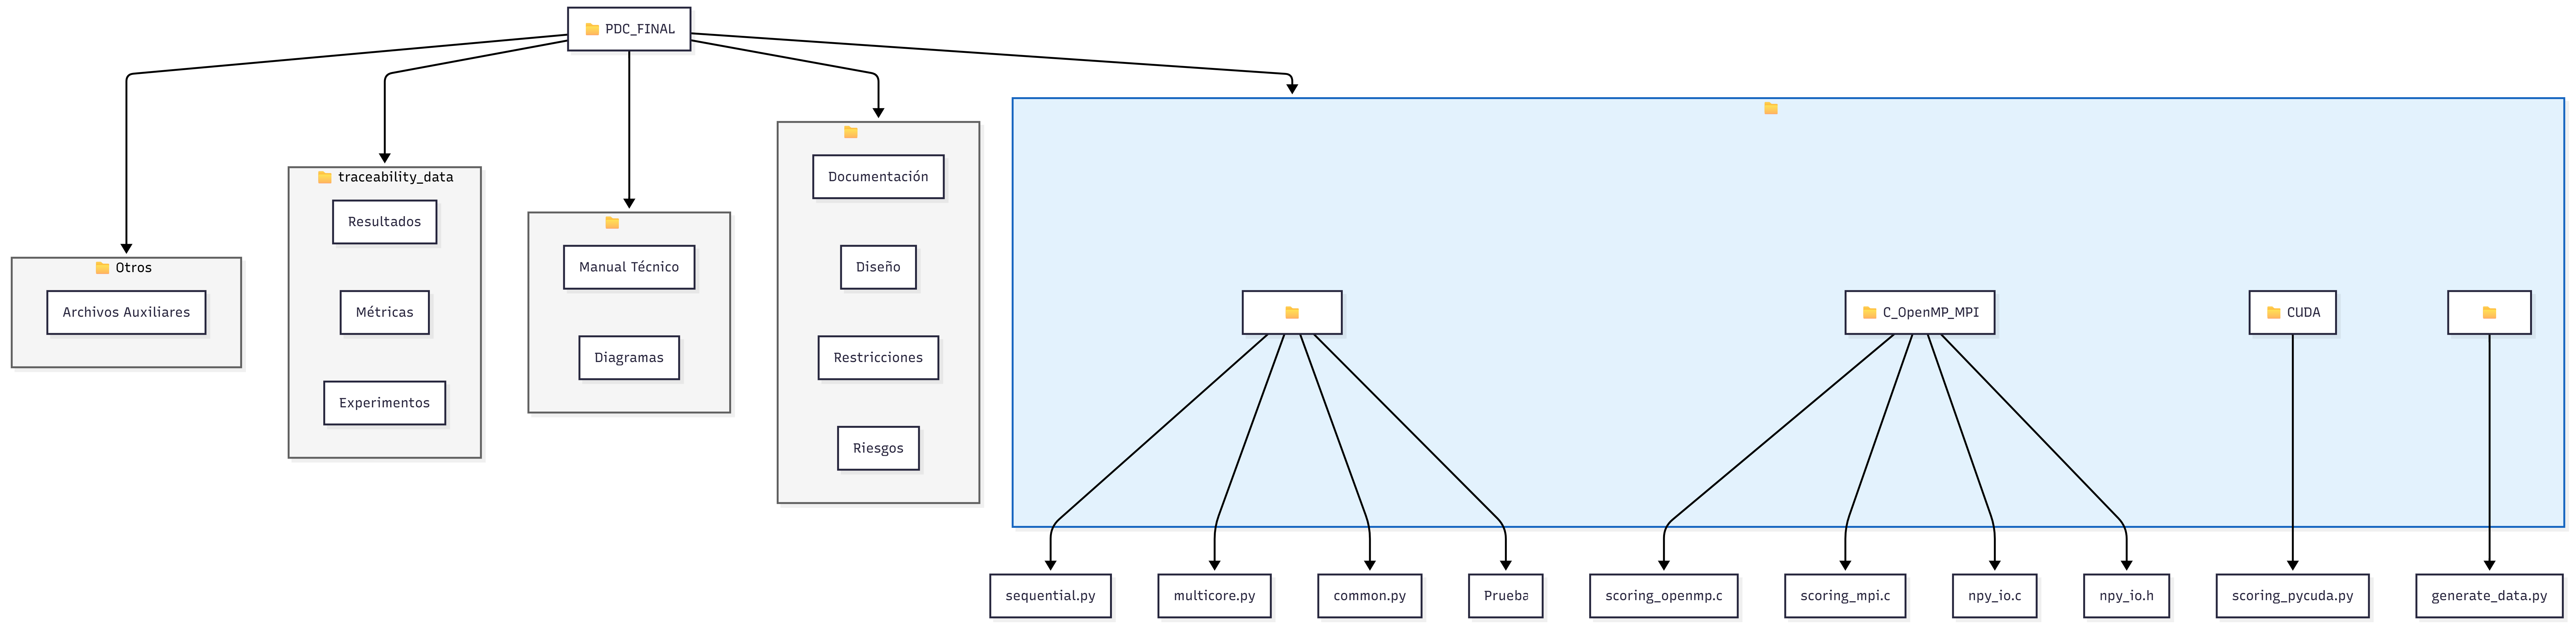
\includegraphics[width=0.95\textwidth]
    {figuras/arquitectura/05_estructura_repositorio.png}
    \caption{Estructura general del repositorio \texttt{PDC\_FINAL}.}
    \label{fig:estructura_repositorio}
\end{figure}

La organización general del proyecto puede resumirse de la siguiente manera:

\begin{lstlisting}[language={}]
PDC_FINAL/
|-- code/
|-- context/
|-- docs/
|-- traceability_data/
`-- others/
\end{lstlisting}

%=========================================================
\section{Correspondencia con la Estructura del Proyecto}

El enunciado original propone una estructura mínima para organizar el desarrollo de las diferentes implementaciones y los experimentos realizados. Conceptualmente dicha organización corresponde a:

\begin{lstlisting}[language={}]
scoring_metagenomico/
|-- data/
|-- python/
|-- C_OpenMP_MPI/
|-- CUDA/
|-- results/
`-- report/
\end{lstlisting}

En el presente proyecto esta organización fue adaptada a una estructura más amplia, integrando los componentes anteriores dentro del directorio \texttt{code} y añadiendo directorios especializados para documentación, trazabilidad y gestión del proyecto. Esta adaptación conserva la separación lógica entre las distintas responsabilidades del sistema, al tiempo que facilita el mantenimiento del repositorio y la incorporación de nuevos componentes.

%=========================================================
\section{Descripción General}

La estructura modular permite separar las diferentes responsabilidades del proyecto, manteniendo un bajo acoplamiento entre sus componentes y facilitando la incorporación de nuevas tecnologías sin modificar la organización existente.

Los directorios principales del repositorio son:

\begin{itemize}
    \item \texttt{code}
    \item \texttt{context}
    \item \texttt{docs}
    \item \texttt{traceability\_data}
    \item \texttt{others}
\end{itemize}

Cada uno cumple una función específica dentro del ciclo de desarrollo del proyecto.

%=========================================================
\section{Directorio \texttt{code}}

El directorio \texttt{code} contiene todas las implementaciones desarrolladas para resolver el problema de optimización. Cada tecnología se encuentra organizada en un subdirectorio independiente, permitiendo comparar fácilmente los diferentes paradigmas de programación utilizados.

%---------------------------------------------------------
\subsection{\texttt{code/python}}

Contiene las implementaciones desarrolladas completamente en Python.

Los archivos principales son:

\begin{itemize}

\item \texttt{sequential.py}: implementación secuencial utilizada como línea base para las comparaciones de rendimiento.

\item \texttt{multicore.py}: implementación paralela utilizando el módulo \texttt{multiprocessing} de Python.

\item \texttt{common.py}: funciones compartidas por las diferentes versiones implementadas en Python.

\item \texttt{tests/}: conjunto de pruebas automatizadas empleadas para verificar el correcto funcionamiento del algoritmo.

\end{itemize}

%---------------------------------------------------------
\subsection{\texttt{code/C\_OpenMP\_MPI}}

Agrupa las implementaciones desarrolladas en lenguaje C para arquitecturas de memoria compartida y memoria distribuida.

Entre los archivos más importantes se encuentran:

\begin{itemize}

\item \texttt{scoring\_openmp.c}: implementación utilizando OpenMP.

\item \texttt{scoring\_mpi.c}: implementación basada en MPI.

\item \texttt{npy\_io.c}: funciones para la lectura de archivos NumPy desde C.

\item \texttt{npy\_io.h}: definiciones y prototipos utilizados por el módulo de lectura.

\item \texttt{Makefile}: automatiza el proceso de compilación de las implementaciones desarrolladas en C.

\end{itemize}

%---------------------------------------------------------
\subsection{\texttt{code/CUDA}}

Este directorio contiene la implementación acelerada mediante GPU.

Actualmente incluye:

\begin{itemize}

\item \texttt{scoring\_pycuda.py}: implementación utilizando PyCUDA para ejecutar el algoritmo sobre dispositivos NVIDIA compatibles con CUDA.

\item \texttt{scoring\_kernel.cu}: kernel CUDA encargado de ejecutar las operaciones paralelas sobre la GPU.

\item \texttt{Makefile}: automatiza la compilación y ejecución de los componentes desarrollados para CUDA.

\end{itemize}

%---------------------------------------------------------
\subsection{\texttt{code/data}}

Contiene los scripts utilizados para generar y preparar los conjuntos de datos empleados durante las pruebas experimentales.

Entre ellos se encuentra:

\begin{itemize}

\item \texttt{generate\_data.py}: generación automática de la matriz de contribución $A$ y del vector de etiquetas $y$ utilizados por todas las implementaciones del proyecto.

\item \texttt{matrix\_A.npy}: almacenamiento de la matriz de contribución generada para la experimentación.

\item \texttt{labels.npy}: almacenamiento de las etiquetas binarias correspondientes a las muestras.

\end{itemize}

El script \texttt{generate\_data.py} permite configurar el número de ítems utilizados durante la generación del conjunto de datos, facilitando la evaluación de la escalabilidad del algoritmo mediante problemas de diferentes tamaños sin necesidad de modificar el código fuente de las implementaciones.

%=========================================================
\section{Directorio \texttt{context}}

El directorio \texttt{context} agrupa la documentación utilizada durante el desarrollo del proyecto.

Su contenido incluye información relacionada con:

\begin{itemize}

\item decisiones de diseño;

\item restricciones técnicas;

\item planificación del proyecto;

\item riesgos identificados;

\item documentación auxiliar utilizada durante el desarrollo.

\end{itemize}

%=========================================================
\section{Directorio \texttt{docs}}

El directorio \texttt{docs} almacena toda la documentación oficial generada durante el proyecto.

Entre los documentos incluidos se encuentran:

\begin{itemize}

\item Manual Técnico.

\item Diagramas de arquitectura.

\item Recursos gráficos empleados en la documentación.

\item Informe técnico final del proyecto.

\end{itemize}

%=========================================================
\section{Directorio \texttt{traceability\_data}}

A diferencia de un registro de trazabilidad experimental tradicional, este directorio almacena la evidencia correspondiente al uso de herramientas de Inteligencia Artificial durante el desarrollo del proyecto, permitiendo documentar de forma transparente en qué etapas y de qué manera se utilizó asistencia basada en IA.

Su contenido incluye:

\begin{itemize}

\item registros de las conversaciones sostenidas con herramientas de IA durante el desarrollo del proyecto;

\item prompts utilizados para la generación o depuración de código;

\item prompts empleados durante la redacción y organización de la documentación técnica;

\item capturas o exportaciones de las sesiones relevantes de interacción con la IA;

\item observaciones sobre las secciones del proyecto en las que se empleó asistencia de IA y el alcance de dicha asistencia.

\end{itemize}

Esta trazabilidad responde a la necesidad de evidenciar de manera explícita el rol desempeñado por las herramientas de IA durante el desarrollo, distinguiendo entre el trabajo realizado de forma autónoma por el equipo y aquel en el cual se contó con apoyo de este tipo de herramientas. De esta forma se favorece la transparencia académica y se facilita la verificación del proceso de desarrollo del proyecto.

%=========================================================
\section{Resultados Experimentales y Automatización}

Con el propósito de garantizar la reproducibilidad de los experimentos, el proyecto incorpora un conjunto de recursos destinados a automatizar la ejecución de todas las implementaciones y registrar de forma homogénea las métricas obtenidas.

Entre los elementos más importantes se encuentran:

\begin{itemize}

\item \texttt{run\_all.sh}: script encargado de ejecutar automáticamente todas las implementaciones disponibles (Python secuencial, Python multicore, OpenMP, MPI y CUDA), recopilar los resultados experimentales y generar los archivos de salida necesarios para el análisis comparativo.

\item \texttt{benchmark.csv}: archivo que almacena las métricas obtenidas durante cada ejecución experimental, incluyendo el tiempo de ejecución, el mejor valor de ROC-AUC encontrado, el speedup y la eficiencia calculada para cada implementación.

\item \texttt{plots/}: directorio destinado al almacenamiento de las gráficas generadas a partir de los resultados experimentales, utilizadas posteriormente en el análisis comparativo presentado en este documento.

\end{itemize}

La automatización de los experimentos permite ejecutar exactamente la misma batería de pruebas sobre todas las implementaciones desarrolladas, garantizando la comparabilidad de los resultados y favoreciendo la reproducibilidad de los experimentos en diferentes plataformas computacionales.

%=========================================================
\section{Directorio \texttt{others}}

El directorio \texttt{others} agrupa archivos auxiliares que no pertenecen directamente al código fuente ni a la documentación principal, pero que resultan útiles durante el desarrollo y mantenimiento del proyecto.

Puede contener herramientas, scripts temporales, recursos adicionales y archivos de apoyo.

%=========================================================
\section{Beneficios de la Organización}

La organización modular adoptada proporciona múltiples ventajas para el desarrollo y evolución del proyecto:

\begin{itemize}

\item separación entre código, documentación y datos;

\item independencia entre las diferentes implementaciones;

\item reutilización de componentes comunes;

\item facilidad para localizar archivos específicos;

\item mantenimiento simplificado del código fuente;

\item incorporación de nuevas tecnologías sin modificar la estructura existente;

\item trazabilidad del uso de herramientas de Inteligencia Artificial durante el desarrollo;

\item reproducibilidad de los resultados obtenidos;

\item automatización de las pruebas experimentales mediante scripts de ejecución;

\item generación centralizada de métricas y resultados comparativos;

\item facilidad para reproducir los experimentos en diferentes plataformas computacionales;

\item escalabilidad para futuras extensiones del proyecto.

\end{itemize}

En conjunto, esta organización proporciona una base sólida para el desarrollo de aplicaciones de computación concurrente y distribuida. La separación entre código fuente, datos, documentación y resultados experimentales facilita tanto el mantenimiento del proyecto como la comparación objetiva entre las diferentes implementaciones desarrolladas. Asimismo, la incorporación de mecanismos de automatización y trazabilidad del uso de IA contribuye a garantizar tanto la reproducibilidad de los experimentos como la transparencia académica del proceso de desarrollo, aspectos fundamentales en proyectos de computación de alto rendimiento y evaluación del desempeño.